\section{Removing reporting delays and weekday effects}%
\label{sec:spatial_reproduction_number_model}
\subsection{Context}
Forecasting the number of new infections that will be reported in the next day, week or month is one of the main tasks of epidemiological monitoring, see \Cref{sec:objectives}. However, as we have observed in \Cref{sec:data}, the data at our hand are contaminated by the reporting process, most notably the week-day effects, reporting delays, and artifacts due to public holidays.
While we can make the influence of these effects small by aggregating data to the weekly level, see \Cref{sec:regional_growth_factor_model}, modeling on the daily level has its merits: this is the smallest timescale data are available at, and so it should provide better predictions if we leverage the full information available. 
% ForecastHubs do weekly forecasting

% use RKI case data for whole country, split by reporting delay
In this section we use the \acrshort{rki} case data discussed in \Cref{sec:data}. As we have seen in \Cref{fig:reporting_delays_cases} \textbf{A} and \Cref{fig:survival_function_rep_tri_incidences}, most delays are less than $4$ days. Thus, ignoring any cases reported with longer delays, we get for any reporting date $t$ four observations, say 
$$
    Y_{t} = \left( Y_{t, 1}, \dots, Y_{t, 4} \right) \in \N^{4}.
$$
Here $Y_{t,\tau}$, $\tau = 1, \dots, 4$, is the number of newly reported cases for reporting date $t$ with delay $\tau$, such that $Y_{t,\cdot} = \sum_{\tau = 1}^4 Y_{t, \tau}$ is the total number of cases reported for reporting date $t$ with delay $\leq 4$. 
Let $\hat p_{t, \tau} = \frac{Y_{t,\tau}}{Y_{t,\cdot}}$ be the empirical delay probability for day $t$ with delay $\tau$. We have already observed in \Cref{fig:reporting_delays_cases}, that $Y_{t, \cdot}$ is subject to weekday effects, but contrary to hospitalizations (\Cref{fig:double_weekday_effect_hosp}), there is no discernible weekday effect for the delay of cases, see \Cref{fig:weekday_effect_delays}.

\begin{figure}
    \resizebox{\textwidth}{!}{%
        % Created by tikzDevice version 0.12.6 on 2024-08-27 13:02:34
% !TEX encoding = UTF-8 Unicode
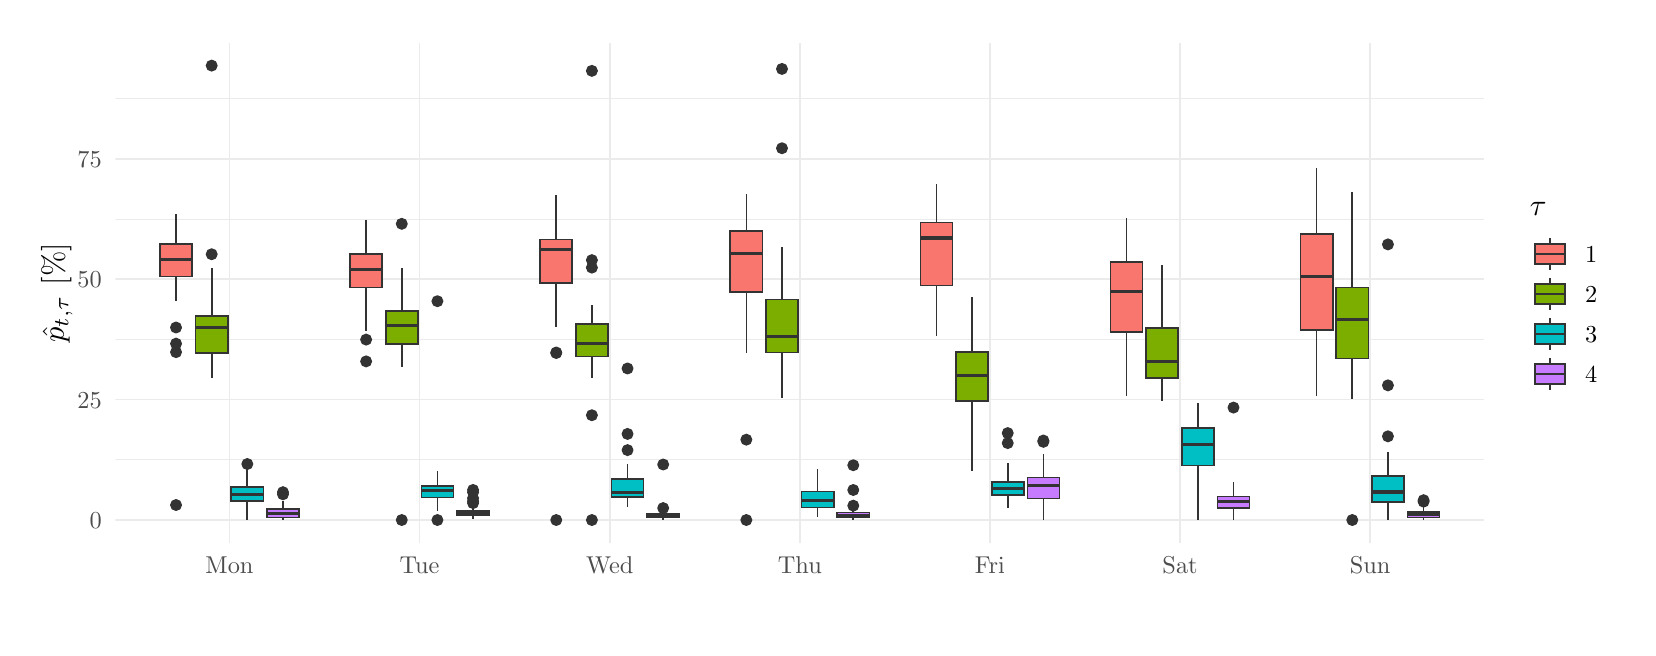
\begin{tikzpicture}[x=1pt,y=1pt]
\definecolor{fillColor}{RGB}{255,255,255}
\path[use as bounding box,fill=fillColor,fill opacity=0.00] (0,0) rectangle (578.16,216.81);
\begin{scope}
\path[clip] ( 31.71, 30.69) rectangle (526.31,211.31);
\definecolor{drawColor}{gray}{0.92}

\path[draw=drawColor,line width= 0.3pt,line join=round] ( 31.71, 60.64) --
	(526.31, 60.64);

\path[draw=drawColor,line width= 0.3pt,line join=round] ( 31.71,104.13) --
	(526.31,104.13);

\path[draw=drawColor,line width= 0.3pt,line join=round] ( 31.71,147.62) --
	(526.31,147.62);

\path[draw=drawColor,line width= 0.3pt,line join=round] ( 31.71,191.11) --
	(526.31,191.11);

\path[draw=drawColor,line width= 0.6pt,line join=round] ( 31.71, 38.90) --
	(526.31, 38.90);

\path[draw=drawColor,line width= 0.6pt,line join=round] ( 31.71, 82.39) --
	(526.31, 82.39);

\path[draw=drawColor,line width= 0.6pt,line join=round] ( 31.71,125.88) --
	(526.31,125.88);

\path[draw=drawColor,line width= 0.6pt,line join=round] ( 31.71,169.36) --
	(526.31,169.36);

\path[draw=drawColor,line width= 0.6pt,line join=round] ( 72.93, 30.69) --
	( 72.93,211.31);

\path[draw=drawColor,line width= 0.6pt,line join=round] (141.62, 30.69) --
	(141.62,211.31);

\path[draw=drawColor,line width= 0.6pt,line join=round] (210.32, 30.69) --
	(210.32,211.31);

\path[draw=drawColor,line width= 0.6pt,line join=round] (279.01, 30.69) --
	(279.01,211.31);

\path[draw=drawColor,line width= 0.6pt,line join=round] (347.70, 30.69) --
	(347.70,211.31);

\path[draw=drawColor,line width= 0.6pt,line join=round] (416.40, 30.69) --
	(416.40,211.31);

\path[draw=drawColor,line width= 0.6pt,line join=round] (485.09, 30.69) --
	(485.09,211.31);
\definecolor{drawColor}{gray}{0.20}
\definecolor{fillColor}{gray}{0.20}

\path[draw=drawColor,line width= 0.4pt,line join=round,line cap=round,fill=fillColor] ( 53.61,108.46) circle (  1.96);

\path[draw=drawColor,line width= 0.4pt,line join=round,line cap=round,fill=fillColor] ( 53.61,102.63) circle (  1.96);

\path[draw=drawColor,line width= 0.4pt,line join=round,line cap=round,fill=fillColor] ( 53.61, 99.56) circle (  1.96);

\path[draw=drawColor,line width= 0.4pt,line join=round,line cap=round,fill=fillColor] ( 53.61, 44.32) circle (  1.96);

\path[draw=drawColor,line width= 0.6pt,line join=round] ( 53.61,138.67) -- ( 53.61,149.60);

\path[draw=drawColor,line width= 0.6pt,line join=round] ( 53.61,126.86) -- ( 53.61,118.04);
\definecolor{fillColor}{RGB}{248,118,109}

\path[draw=drawColor,line width= 0.6pt,fill=fillColor] ( 47.81,138.67) --
	( 47.81,126.86) --
	( 59.40,126.86) --
	( 59.40,138.67) --
	( 47.81,138.67) --
	cycle;

\path[draw=drawColor,line width= 1.1pt] ( 47.81,133.04) -- ( 59.40,133.04);
\definecolor{fillColor}{gray}{0.20}

\path[draw=drawColor,line width= 0.4pt,line join=round,line cap=round,fill=fillColor] ( 66.49,134.94) circle (  1.96);

\path[draw=drawColor,line width= 0.4pt,line join=round,line cap=round,fill=fillColor] ( 66.49,203.10) circle (  1.96);

\path[draw=drawColor,line width= 0.6pt,line join=round] ( 66.49,112.55) -- ( 66.49,129.94);

\path[draw=drawColor,line width= 0.6pt,line join=round] ( 66.49, 99.20) -- ( 66.49, 90.37);
\definecolor{fillColor}{RGB}{124,174,0}

\path[draw=drawColor,line width= 0.6pt,fill=fillColor] ( 60.69,112.55) --
	( 60.69, 99.20) --
	( 72.28, 99.20) --
	( 72.28,112.55) --
	( 60.69,112.55) --
	cycle;

\path[draw=drawColor,line width= 1.1pt] ( 60.69,108.36) -- ( 72.28,108.36);
\definecolor{fillColor}{gray}{0.20}

\path[draw=drawColor,line width= 0.4pt,line join=round,line cap=round,fill=fillColor] ( 79.37, 59.14) circle (  1.96);

\path[draw=drawColor,line width= 0.6pt,line join=round] ( 79.37, 50.73) -- ( 79.37, 58.08);

\path[draw=drawColor,line width= 0.6pt,line join=round] ( 79.37, 45.68) -- ( 79.37, 38.90);
\definecolor{fillColor}{RGB}{0,191,196}

\path[draw=drawColor,line width= 0.6pt,fill=fillColor] ( 73.57, 50.73) --
	( 73.57, 45.68) --
	( 85.16, 45.68) --
	( 85.16, 50.73) --
	( 73.57, 50.73) --
	cycle;

\path[draw=drawColor,line width= 1.1pt] ( 73.57, 48.05) -- ( 85.16, 48.05);
\definecolor{fillColor}{gray}{0.20}

\path[draw=drawColor,line width= 0.4pt,line join=round,line cap=round,fill=fillColor] ( 92.25, 48.96) circle (  1.96);

\path[draw=drawColor,line width= 0.4pt,line join=round,line cap=round,fill=fillColor] ( 92.25, 48.19) circle (  1.96);

\path[draw=drawColor,line width= 0.6pt,line join=round] ( 92.25, 42.79) -- ( 92.25, 45.95);

\path[draw=drawColor,line width= 0.6pt,line join=round] ( 92.25, 39.80) -- ( 92.25, 38.90);
\definecolor{fillColor}{RGB}{199,124,255}

\path[draw=drawColor,line width= 0.6pt,fill=fillColor] ( 86.45, 42.79) --
	( 86.45, 39.80) --
	( 98.04, 39.80) --
	( 98.04, 42.79) --
	( 86.45, 42.79) --
	cycle;

\path[draw=drawColor,line width= 1.1pt] ( 86.45, 41.36) -- ( 98.04, 41.36);
\definecolor{fillColor}{gray}{0.20}

\path[draw=drawColor,line width= 0.4pt,line join=round,line cap=round,fill=fillColor] (122.30,104.09) circle (  1.96);

\path[draw=drawColor,line width= 0.4pt,line join=round,line cap=round,fill=fillColor] (122.30, 96.22) circle (  1.96);

\path[draw=drawColor,line width= 0.6pt,line join=round] (122.30,135.14) -- (122.30,147.36);

\path[draw=drawColor,line width= 0.6pt,line join=round] (122.30,122.87) -- (122.30,107.08);
\definecolor{fillColor}{RGB}{248,118,109}

\path[draw=drawColor,line width= 0.6pt,fill=fillColor] (116.51,135.14) --
	(116.51,122.87) --
	(128.10,122.87) --
	(128.10,135.14) --
	(116.51,135.14) --
	cycle;

\path[draw=drawColor,line width= 1.1pt] (116.51,129.28) -- (128.10,129.28);
\definecolor{fillColor}{gray}{0.20}

\path[draw=drawColor,line width= 0.4pt,line join=round,line cap=round,fill=fillColor] (135.18,145.93) circle (  1.96);

\path[draw=drawColor,line width= 0.4pt,line join=round,line cap=round,fill=fillColor] (135.18, 38.90) circle (  1.96);

\path[draw=drawColor,line width= 0.6pt,line join=round] (135.18,114.54) -- (135.18,130.07);

\path[draw=drawColor,line width= 0.6pt,line join=round] (135.18,102.42) -- (135.18, 94.15);
\definecolor{fillColor}{RGB}{124,174,0}

\path[draw=drawColor,line width= 0.6pt,fill=fillColor] (129.39,114.54) --
	(129.39,102.42) --
	(140.98,102.42) --
	(140.98,114.54) --
	(129.39,114.54) --
	cycle;

\path[draw=drawColor,line width= 1.1pt] (129.39,109.02) -- (140.98,109.02);
\definecolor{fillColor}{gray}{0.20}

\path[draw=drawColor,line width= 0.4pt,line join=round,line cap=round,fill=fillColor] (148.06,117.97) circle (  1.96);

\path[draw=drawColor,line width= 0.4pt,line join=round,line cap=round,fill=fillColor] (148.06, 38.90) circle (  1.96);

\path[draw=drawColor,line width= 0.6pt,line join=round] (148.06, 51.13) -- (148.06, 56.72);

\path[draw=drawColor,line width= 0.6pt,line join=round] (148.06, 47.00) -- (148.06, 42.04);
\definecolor{fillColor}{RGB}{0,191,196}

\path[draw=drawColor,line width= 0.6pt,fill=fillColor] (142.27, 51.13) --
	(142.27, 47.00) --
	(153.86, 47.00) --
	(153.86, 51.13) --
	(142.27, 51.13) --
	cycle;

\path[draw=drawColor,line width= 1.1pt] (142.27, 49.43) -- (153.86, 49.43);
\definecolor{fillColor}{gray}{0.20}

\path[draw=drawColor,line width= 0.4pt,line join=round,line cap=round,fill=fillColor] (160.94, 48.93) circle (  1.96);

\path[draw=drawColor,line width= 0.4pt,line join=round,line cap=round,fill=fillColor] (160.94, 49.77) circle (  1.96);

\path[draw=drawColor,line width= 0.4pt,line join=round,line cap=round,fill=fillColor] (160.94, 46.79) circle (  1.96);

\path[draw=drawColor,line width= 0.4pt,line join=round,line cap=round,fill=fillColor] (160.94, 45.01) circle (  1.96);

\path[draw=drawColor,line width= 0.4pt,line join=round,line cap=round,fill=fillColor] (160.94, 45.72) circle (  1.96);

\path[draw=drawColor,line width= 0.6pt,line join=round] (160.94, 42.16) -- (160.94, 44.42);

\path[draw=drawColor,line width= 0.6pt,line join=round] (160.94, 40.56) -- (160.94, 39.10);
\definecolor{fillColor}{RGB}{199,124,255}

\path[draw=drawColor,line width= 0.6pt,fill=fillColor] (155.15, 42.16) --
	(155.15, 40.56) --
	(166.74, 40.56) --
	(166.74, 42.16) --
	(155.15, 42.16) --
	cycle;

\path[draw=drawColor,line width= 1.1pt] (155.15, 41.22) -- (166.74, 41.22);
\definecolor{fillColor}{gray}{0.20}

\path[draw=drawColor,line width= 0.4pt,line join=round,line cap=round,fill=fillColor] (191.00, 99.43) circle (  1.96);

\path[draw=drawColor,line width= 0.4pt,line join=round,line cap=round,fill=fillColor] (191.00, 99.25) circle (  1.96);

\path[draw=drawColor,line width= 0.4pt,line join=round,line cap=round,fill=fillColor] (191.00, 38.90) circle (  1.96);

\path[draw=drawColor,line width= 0.6pt,line join=round] (191.00,140.27) -- (191.00,156.21);

\path[draw=drawColor,line width= 0.6pt,line join=round] (191.00,124.46) -- (191.00,108.72);
\definecolor{fillColor}{RGB}{248,118,109}

\path[draw=drawColor,line width= 0.6pt,fill=fillColor] (185.20,140.27) --
	(185.20,124.46) --
	(196.79,124.46) --
	(196.79,140.27) --
	(185.20,140.27) --
	cycle;

\path[draw=drawColor,line width= 1.1pt] (185.20,136.51) -- (196.79,136.51);
\definecolor{fillColor}{gray}{0.20}

\path[draw=drawColor,line width= 0.4pt,line join=round,line cap=round,fill=fillColor] (203.88,130.11) circle (  1.96);

\path[draw=drawColor,line width= 0.4pt,line join=round,line cap=round,fill=fillColor] (203.88,132.81) circle (  1.96);

\path[draw=drawColor,line width= 0.4pt,line join=round,line cap=round,fill=fillColor] (203.88, 76.77) circle (  1.96);

\path[draw=drawColor,line width= 0.4pt,line join=round,line cap=round,fill=fillColor] (203.88,201.20) circle (  1.96);

\path[draw=drawColor,line width= 0.4pt,line join=round,line cap=round,fill=fillColor] (203.88, 38.90) circle (  1.96);

\path[draw=drawColor,line width= 0.6pt,line join=round] (203.88,109.68) -- (203.88,116.57);

\path[draw=drawColor,line width= 0.6pt,line join=round] (203.88, 98.01) -- (203.88, 90.22);
\definecolor{fillColor}{RGB}{124,174,0}

\path[draw=drawColor,line width= 0.6pt,fill=fillColor] (198.08,109.68) --
	(198.08, 98.01) --
	(209.67, 98.01) --
	(209.67,109.68) --
	(198.08,109.68) --
	cycle;

\path[draw=drawColor,line width= 1.1pt] (198.08,102.76) -- (209.67,102.76);
\definecolor{fillColor}{gray}{0.20}

\path[draw=drawColor,line width= 0.4pt,line join=round,line cap=round,fill=fillColor] (216.76, 64.16) circle (  1.96);

\path[draw=drawColor,line width= 0.4pt,line join=round,line cap=round,fill=fillColor] (216.76, 70.01) circle (  1.96);

\path[draw=drawColor,line width= 0.4pt,line join=round,line cap=round,fill=fillColor] (216.76, 93.66) circle (  1.96);

\path[draw=drawColor,line width= 0.6pt,line join=round] (216.76, 53.72) -- (216.76, 59.24);

\path[draw=drawColor,line width= 0.6pt,line join=round] (216.76, 47.22) -- (216.76, 43.53);
\definecolor{fillColor}{RGB}{0,191,196}

\path[draw=drawColor,line width= 0.6pt,fill=fillColor] (210.96, 53.72) --
	(210.96, 47.22) --
	(222.55, 47.22) --
	(222.55, 53.72) --
	(210.96, 53.72) --
	cycle;

\path[draw=drawColor,line width= 1.1pt] (210.96, 48.99) -- (222.55, 48.99);
\definecolor{fillColor}{gray}{0.20}

\path[draw=drawColor,line width= 0.4pt,line join=round,line cap=round,fill=fillColor] (229.64, 58.96) circle (  1.96);

\path[draw=drawColor,line width= 0.4pt,line join=round,line cap=round,fill=fillColor] (229.64, 43.21) circle (  1.96);

\path[draw=drawColor,line width= 0.6pt,line join=round] (229.64, 41.12) -- (229.64, 42.34);

\path[draw=drawColor,line width= 0.6pt,line join=round] (229.64, 39.90) -- (229.64, 38.90);
\definecolor{fillColor}{RGB}{199,124,255}

\path[draw=drawColor,line width= 0.6pt,fill=fillColor] (223.84, 41.12) --
	(223.84, 39.90) --
	(235.43, 39.90) --
	(235.43, 41.12) --
	(223.84, 41.12) --
	cycle;

\path[draw=drawColor,line width= 1.1pt] (223.84, 40.45) -- (235.43, 40.45);
\definecolor{fillColor}{gray}{0.20}

\path[draw=drawColor,line width= 0.4pt,line join=round,line cap=round,fill=fillColor] (259.69, 67.93) circle (  1.96);

\path[draw=drawColor,line width= 0.4pt,line join=round,line cap=round,fill=fillColor] (259.69, 38.90) circle (  1.96);

\path[draw=drawColor,line width= 0.6pt,line join=round] (259.69,143.45) -- (259.69,156.54);

\path[draw=drawColor,line width= 0.6pt,line join=round] (259.69,121.36) -- (259.69, 99.37);
\definecolor{fillColor}{RGB}{248,118,109}

\path[draw=drawColor,line width= 0.6pt,fill=fillColor] (253.89,143.45) --
	(253.89,121.36) --
	(265.49,121.36) --
	(265.49,143.45) --
	(253.89,143.45) --
	cycle;

\path[draw=drawColor,line width= 1.1pt] (253.89,135.11) -- (265.49,135.11);
\definecolor{fillColor}{gray}{0.20}

\path[draw=drawColor,line width= 0.4pt,line join=round,line cap=round,fill=fillColor] (272.57,173.24) circle (  1.96);

\path[draw=drawColor,line width= 0.4pt,line join=round,line cap=round,fill=fillColor] (272.57,201.90) circle (  1.96);

\path[draw=drawColor,line width= 0.6pt,line join=round] (272.57,118.55) -- (272.57,137.57);

\path[draw=drawColor,line width= 0.6pt,line join=round] (272.57, 99.49) -- (272.57, 82.99);
\definecolor{fillColor}{RGB}{124,174,0}

\path[draw=drawColor,line width= 0.6pt,fill=fillColor] (266.77,118.55) --
	(266.77, 99.49) --
	(278.37, 99.49) --
	(278.37,118.55) --
	(266.77,118.55) --
	cycle;

\path[draw=drawColor,line width= 1.1pt] (266.77,105.38) -- (278.37,105.38);

\path[draw=drawColor,line width= 0.6pt,line join=round] (285.45, 49.23) -- (285.45, 57.20);

\path[draw=drawColor,line width= 0.6pt,line join=round] (285.45, 43.42) -- (285.45, 39.88);
\definecolor{fillColor}{RGB}{0,191,196}

\path[draw=drawColor,line width= 0.6pt,fill=fillColor] (279.65, 49.23) --
	(279.65, 43.42) --
	(291.25, 43.42) --
	(291.25, 49.23) --
	(279.65, 49.23) --
	cycle;

\path[draw=drawColor,line width= 1.1pt] (279.65, 45.80) -- (291.25, 45.80);
\definecolor{fillColor}{gray}{0.20}

\path[draw=drawColor,line width= 0.4pt,line join=round,line cap=round,fill=fillColor] (298.33, 44.09) circle (  1.96);

\path[draw=drawColor,line width= 0.4pt,line join=round,line cap=round,fill=fillColor] (298.33, 49.75) circle (  1.96);

\path[draw=drawColor,line width= 0.4pt,line join=round,line cap=round,fill=fillColor] (298.33, 58.70) circle (  1.96);

\path[draw=drawColor,line width= 0.6pt,line join=round] (298.33, 41.66) -- (298.33, 43.75);

\path[draw=drawColor,line width= 0.6pt,line join=round] (298.33, 40.06) -- (298.33, 38.90);
\definecolor{fillColor}{RGB}{199,124,255}

\path[draw=drawColor,line width= 0.6pt,fill=fillColor] (292.53, 41.66) --
	(292.53, 40.06) --
	(304.13, 40.06) --
	(304.13, 41.66) --
	(292.53, 41.66) --
	cycle;

\path[draw=drawColor,line width= 1.1pt] (292.53, 40.70) -- (304.13, 40.70);

\path[draw=drawColor,line width= 0.6pt,line join=round] (328.38,146.40) -- (328.38,160.14);

\path[draw=drawColor,line width= 0.6pt,line join=round] (328.38,123.66) -- (328.38,105.35);
\definecolor{fillColor}{RGB}{248,118,109}

\path[draw=drawColor,line width= 0.6pt,fill=fillColor] (322.59,146.40) --
	(322.59,123.66) --
	(334.18,123.66) --
	(334.18,146.40) --
	(322.59,146.40) --
	cycle;

\path[draw=drawColor,line width= 1.1pt] (322.59,140.80) -- (334.18,140.80);

\path[draw=drawColor,line width= 0.6pt,line join=round] (341.26, 99.65) -- (341.26,119.60);

\path[draw=drawColor,line width= 0.6pt,line join=round] (341.26, 81.98) -- (341.26, 56.47);
\definecolor{fillColor}{RGB}{124,174,0}

\path[draw=drawColor,line width= 0.6pt,fill=fillColor] (335.47, 99.65) --
	(335.47, 81.98) --
	(347.06, 81.98) --
	(347.06, 99.65) --
	(335.47, 99.65) --
	cycle;

\path[draw=drawColor,line width= 1.1pt] (335.47, 91.20) -- (347.06, 91.20);
\definecolor{fillColor}{gray}{0.20}

\path[draw=drawColor,line width= 0.4pt,line join=round,line cap=round,fill=fillColor] (354.14, 66.70) circle (  1.96);

\path[draw=drawColor,line width= 0.4pt,line join=round,line cap=round,fill=fillColor] (354.14, 70.31) circle (  1.96);

\path[draw=drawColor,line width= 0.6pt,line join=round] (354.14, 52.68) -- (354.14, 59.36);

\path[draw=drawColor,line width= 0.6pt,line join=round] (354.14, 47.97) -- (354.14, 43.12);
\definecolor{fillColor}{RGB}{0,191,196}

\path[draw=drawColor,line width= 0.6pt,fill=fillColor] (348.35, 52.68) --
	(348.35, 47.97) --
	(359.94, 47.97) --
	(359.94, 52.68) --
	(348.35, 52.68) --
	cycle;

\path[draw=drawColor,line width= 1.1pt] (348.35, 50.20) -- (359.94, 50.20);
\definecolor{fillColor}{gray}{0.20}

\path[draw=drawColor,line width= 0.4pt,line join=round,line cap=round,fill=fillColor] (367.02, 67.15) circle (  1.96);

\path[draw=drawColor,line width= 0.4pt,line join=round,line cap=round,fill=fillColor] (367.02, 67.63) circle (  1.96);

\path[draw=drawColor,line width= 0.6pt,line join=round] (367.02, 54.31) -- (367.02, 62.79);

\path[draw=drawColor,line width= 0.6pt,line join=round] (367.02, 46.69) -- (367.02, 38.90);
\definecolor{fillColor}{RGB}{199,124,255}

\path[draw=drawColor,line width= 0.6pt,fill=fillColor] (361.23, 54.31) --
	(361.23, 46.69) --
	(372.82, 46.69) --
	(372.82, 54.31) --
	(361.23, 54.31) --
	cycle;

\path[draw=drawColor,line width= 1.1pt] (361.23, 51.51) -- (372.82, 51.51);

\path[draw=drawColor,line width= 0.6pt,line join=round] (397.08,132.11) -- (397.08,147.94);

\path[draw=drawColor,line width= 0.6pt,line join=round] (397.08,106.78) -- (397.08, 83.54);
\definecolor{fillColor}{RGB}{248,118,109}

\path[draw=drawColor,line width= 0.6pt,fill=fillColor] (391.28,132.11) --
	(391.28,106.78) --
	(402.87,106.78) --
	(402.87,132.11) --
	(391.28,132.11) --
	cycle;

\path[draw=drawColor,line width= 1.1pt] (391.28,121.56) -- (402.87,121.56);

\path[draw=drawColor,line width= 0.6pt,line join=round] (409.96,108.34) -- (409.96,131.15);

\path[draw=drawColor,line width= 0.6pt,line join=round] (409.96, 90.28) -- (409.96, 81.74);
\definecolor{fillColor}{RGB}{124,174,0}

\path[draw=drawColor,line width= 0.6pt,fill=fillColor] (404.16,108.34) --
	(404.16, 90.28) --
	(415.75, 90.28) --
	(415.75,108.34) --
	(404.16,108.34) --
	cycle;

\path[draw=drawColor,line width= 1.1pt] (404.16, 96.26) -- (415.75, 96.26);

\path[draw=drawColor,line width= 0.6pt,line join=round] (422.84, 72.12) -- (422.84, 81.35);

\path[draw=drawColor,line width= 0.6pt,line join=round] (422.84, 58.64) -- (422.84, 38.90);
\definecolor{fillColor}{RGB}{0,191,196}

\path[draw=drawColor,line width= 0.6pt,fill=fillColor] (417.04, 72.12) --
	(417.04, 58.64) --
	(428.63, 58.64) --
	(428.63, 72.12) --
	(417.04, 72.12) --
	cycle;

\path[draw=drawColor,line width= 1.1pt] (417.04, 66.08) -- (428.63, 66.08);
\definecolor{fillColor}{gray}{0.20}

\path[draw=drawColor,line width= 0.4pt,line join=round,line cap=round,fill=fillColor] (435.72, 79.53) circle (  1.96);

\path[draw=drawColor,line width= 0.6pt,line join=round] (435.72, 47.42) -- (435.72, 52.60);

\path[draw=drawColor,line width= 0.6pt,line join=round] (435.72, 43.26) -- (435.72, 38.90);
\definecolor{fillColor}{RGB}{199,124,255}

\path[draw=drawColor,line width= 0.6pt,fill=fillColor] (429.92, 47.42) --
	(429.92, 43.26) --
	(441.51, 43.26) --
	(441.51, 47.42) --
	(429.92, 47.42) --
	cycle;

\path[draw=drawColor,line width= 1.1pt] (429.92, 45.46) -- (441.51, 45.46);

\path[draw=drawColor,line width= 0.6pt,line join=round] (465.77,142.34) -- (465.77,165.99);

\path[draw=drawColor,line width= 0.6pt,line join=round] (465.77,107.53) -- (465.77, 83.76);
\definecolor{fillColor}{RGB}{248,118,109}

\path[draw=drawColor,line width= 0.6pt,fill=fillColor] (459.97,142.34) --
	(459.97,107.53) --
	(471.57,107.53) --
	(471.57,142.34) --
	(459.97,142.34) --
	cycle;

\path[draw=drawColor,line width= 1.1pt] (459.97,126.95) -- (471.57,126.95);
\definecolor{fillColor}{gray}{0.20}

\path[draw=drawColor,line width= 0.4pt,line join=round,line cap=round,fill=fillColor] (478.65, 38.90) circle (  1.96);

\path[draw=drawColor,line width= 0.6pt,line join=round] (478.65,122.90) -- (478.65,157.31);

\path[draw=drawColor,line width= 0.6pt,line join=round] (478.65, 97.22) -- (478.65, 82.58);
\definecolor{fillColor}{RGB}{124,174,0}

\path[draw=drawColor,line width= 0.6pt,fill=fillColor] (472.85,122.90) --
	(472.85, 97.22) --
	(484.45, 97.22) --
	(484.45,122.90) --
	(472.85,122.90) --
	cycle;

\path[draw=drawColor,line width= 1.1pt] (472.85,111.47) -- (484.45,111.47);
\definecolor{fillColor}{gray}{0.20}

\path[draw=drawColor,line width= 0.4pt,line join=round,line cap=round,fill=fillColor] (491.53, 87.56) circle (  1.96);

\path[draw=drawColor,line width= 0.4pt,line join=round,line cap=round,fill=fillColor] (491.53,138.49) circle (  1.96);

\path[draw=drawColor,line width= 0.4pt,line join=round,line cap=round,fill=fillColor] (491.53, 69.14) circle (  1.96);

\path[draw=drawColor,line width= 0.6pt,line join=round] (491.53, 54.70) -- (491.53, 63.51);

\path[draw=drawColor,line width= 0.6pt,line join=round] (491.53, 45.38) -- (491.53, 38.90);
\definecolor{fillColor}{RGB}{0,191,196}

\path[draw=drawColor,line width= 0.6pt,fill=fillColor] (485.73, 54.70) --
	(485.73, 45.38) --
	(497.33, 45.38) --
	(497.33, 54.70) --
	(485.73, 54.70) --
	cycle;

\path[draw=drawColor,line width= 1.1pt] (485.73, 49.03) -- (497.33, 49.03);
\definecolor{fillColor}{gray}{0.20}

\path[draw=drawColor,line width= 0.4pt,line join=round,line cap=round,fill=fillColor] (504.41, 46.07) circle (  1.96);

\path[draw=drawColor,line width= 0.4pt,line join=round,line cap=round,fill=fillColor] (504.41, 45.54) circle (  1.96);

\path[draw=drawColor,line width= 0.6pt,line join=round] (504.41, 41.73) -- (504.41, 43.83);

\path[draw=drawColor,line width= 0.6pt,line join=round] (504.41, 39.85) -- (504.41, 38.90);
\definecolor{fillColor}{RGB}{199,124,255}

\path[draw=drawColor,line width= 0.6pt,fill=fillColor] (498.61, 41.73) --
	(498.61, 39.85) --
	(510.21, 39.85) --
	(510.21, 41.73) --
	(498.61, 41.73) --
	cycle;

\path[draw=drawColor,line width= 1.1pt] (498.61, 40.90) -- (510.21, 40.90);
\end{scope}
\begin{scope}
\path[clip] (  0.00,  0.00) rectangle (578.16,216.81);
\definecolor{drawColor}{gray}{0.30}

\node[text=drawColor,anchor=base east,inner sep=0pt, outer sep=0pt, scale=  0.88] at ( 26.76, 35.87) {0};

\node[text=drawColor,anchor=base east,inner sep=0pt, outer sep=0pt, scale=  0.88] at ( 26.76, 79.36) {25};

\node[text=drawColor,anchor=base east,inner sep=0pt, outer sep=0pt, scale=  0.88] at ( 26.76,122.84) {50};

\node[text=drawColor,anchor=base east,inner sep=0pt, outer sep=0pt, scale=  0.88] at ( 26.76,166.33) {75};
\end{scope}
\begin{scope}
\path[clip] (  0.00,  0.00) rectangle (578.16,216.81);
\definecolor{drawColor}{gray}{0.30}

\node[text=drawColor,anchor=base,inner sep=0pt, outer sep=0pt, scale=  0.88] at ( 72.93, 19.68) {Mon};

\node[text=drawColor,anchor=base,inner sep=0pt, outer sep=0pt, scale=  0.88] at (141.62, 19.68) {Tue};

\node[text=drawColor,anchor=base,inner sep=0pt, outer sep=0pt, scale=  0.88] at (210.32, 19.68) {Wed};

\node[text=drawColor,anchor=base,inner sep=0pt, outer sep=0pt, scale=  0.88] at (279.01, 19.68) {Thu};

\node[text=drawColor,anchor=base,inner sep=0pt, outer sep=0pt, scale=  0.88] at (347.70, 19.68) {Fri};

\node[text=drawColor,anchor=base,inner sep=0pt, outer sep=0pt, scale=  0.88] at (416.40, 19.68) {Sat};

\node[text=drawColor,anchor=base,inner sep=0pt, outer sep=0pt, scale=  0.88] at (485.09, 19.68) {Sun};
\end{scope}
\begin{scope}
\path[clip] (  0.00,  0.00) rectangle (578.16,216.81);
\definecolor{drawColor}{RGB}{0,0,0}

\node[text=drawColor,rotate= 90.00,anchor=base,inner sep=0pt, outer sep=0pt, scale=  1.10] at ( 13.08,121.00) {$\hat p_{t, \tau}$ [\%]};
\end{scope}
\begin{scope}
\path[clip] (  0.00,  0.00) rectangle (578.16,216.81);
\definecolor{drawColor}{RGB}{0,0,0}

\node[text=drawColor,anchor=base west,inner sep=0pt, outer sep=0pt, scale=  1.10] at (542.81,148.87) {$\tau$};
\end{scope}
\begin{scope}
\path[clip] (  0.00,  0.00) rectangle (578.16,216.81);
\definecolor{drawColor}{gray}{0.20}

\path[draw=drawColor,line width= 0.6pt] (550.03,129.29) --
	(550.03,131.46);

\path[draw=drawColor,line width= 0.6pt] (550.03,138.69) --
	(550.03,140.85);
\definecolor{fillColor}{RGB}{248,118,109}

\path[draw=drawColor,line width= 0.6pt,fill=fillColor] (544.61,131.46) rectangle (555.45,138.69);

\path[draw=drawColor,line width= 0.6pt] (544.61,135.07) --
	(555.45,135.07);
\end{scope}
\begin{scope}
\path[clip] (  0.00,  0.00) rectangle (578.16,216.81);
\definecolor{drawColor}{gray}{0.20}

\path[draw=drawColor,line width= 0.6pt] (550.03,114.84) --
	(550.03,117.00);

\path[draw=drawColor,line width= 0.6pt] (550.03,124.23) --
	(550.03,126.40);
\definecolor{fillColor}{RGB}{124,174,0}

\path[draw=drawColor,line width= 0.6pt,fill=fillColor] (544.61,117.00) rectangle (555.45,124.23);

\path[draw=drawColor,line width= 0.6pt] (544.61,120.62) --
	(555.45,120.62);
\end{scope}
\begin{scope}
\path[clip] (  0.00,  0.00) rectangle (578.16,216.81);
\definecolor{drawColor}{gray}{0.20}

\path[draw=drawColor,line width= 0.6pt] (550.03,100.38) --
	(550.03,102.55);

\path[draw=drawColor,line width= 0.6pt] (550.03,109.78) --
	(550.03,111.95);
\definecolor{fillColor}{RGB}{0,191,196}

\path[draw=drawColor,line width= 0.6pt,fill=fillColor] (544.61,102.55) rectangle (555.45,109.78);

\path[draw=drawColor,line width= 0.6pt] (544.61,106.16) --
	(555.45,106.16);
\end{scope}
\begin{scope}
\path[clip] (  0.00,  0.00) rectangle (578.16,216.81);
\definecolor{drawColor}{gray}{0.20}

\path[draw=drawColor,line width= 0.6pt] (550.03, 85.93) --
	(550.03, 88.10);

\path[draw=drawColor,line width= 0.6pt] (550.03, 95.32) --
	(550.03, 97.49);
\definecolor{fillColor}{RGB}{199,124,255}

\path[draw=drawColor,line width= 0.6pt,fill=fillColor] (544.61, 88.10) rectangle (555.45, 95.32);

\path[draw=drawColor,line width= 0.6pt] (544.61, 91.71) --
	(555.45, 91.71);
\end{scope}
\begin{scope}
\path[clip] (  0.00,  0.00) rectangle (578.16,216.81);
\definecolor{drawColor}{RGB}{0,0,0}

\node[text=drawColor,anchor=base west,inner sep=0pt, outer sep=0pt, scale=  0.88] at (562.76,132.04) {1};
\end{scope}
\begin{scope}
\path[clip] (  0.00,  0.00) rectangle (578.16,216.81);
\definecolor{drawColor}{RGB}{0,0,0}

\node[text=drawColor,anchor=base west,inner sep=0pt, outer sep=0pt, scale=  0.88] at (562.76,117.59) {2};
\end{scope}
\begin{scope}
\path[clip] (  0.00,  0.00) rectangle (578.16,216.81);
\definecolor{drawColor}{RGB}{0,0,0}

\node[text=drawColor,anchor=base west,inner sep=0pt, outer sep=0pt, scale=  0.88] at (562.76,103.13) {3};
\end{scope}
\begin{scope}
\path[clip] (  0.00,  0.00) rectangle (578.16,216.81);
\definecolor{drawColor}{RGB}{0,0,0}

\node[text=drawColor,anchor=base west,inner sep=0pt, outer sep=0pt, scale=  0.88] at (562.76, 88.68) {4};
\end{scope}
\end{tikzpicture}
%
    }
    \caption{Box plots of delay probabilities $\hat p_{t,\tau}$ by weekday of case reporting date $t$. While there is a small difference in delays between, e.g., Saturday and other days for $\tau = 3$, the differences are small.}
    \label{fig:weekday_effect_delays}
\end{figure}

To produce accurate forecasts of the daily number of reported cases, we will construct a \acrshort{ssm} that allows to account for these delays, as well as the weekday effects and dynamics of the incidences. With this model, we will then perform short-term forecasts for the case incidence in Germany, including prediction intervals. To assess the performance of our method, we compare the results to those produced in the \acrfull{ecdc}'s ForecastHub \citep{Sherratt2022Predictive}.
\todo{also remove reporting artifacts at christmas?}

\subsection{Model}

To model the development of cases over time, we start with the exponential growth equation \Cref{eq:exponential-growth-time-varying}. Let $I_{t}$ be the total unknown number of cases for reporting date $t$. Ignoring variation around the mean, the exponential growth ansatz gives 
$$
    \log I_{t + 1} \approx \log \rho_{t + 1}  + \log I_{t}
$$
for the growth factor $\rho_{t}$ on day $t$. It is then sensible to assume that the growth factor $\rho_{t}$ performs a random walk on the log-scale, as we would expect large day-to-day variation of $\rho_{t}$ for large values, and small variation for small values, i.e. multiplicative, rather than additive, day-to-day changes. Thus, we assume that 
$$
    \log \rho_{t + 1} = \rho_{t} + \varepsilon_{t + 1, \rho}
$$
for $\varepsilon_{t + 1,\rho} \sim \mathcal N(0, \sigma^{2}_\rho)$. To incorporate week-day effects, consider a weekly seasonal component 
$$
    \log W_{t + 1} = - \sum_{s = 0}^{5} \log W_{t - s} + \varepsilon_{t + 1, W},
$$
for $\varepsilon_{t + 1, W} \sim \mathcal N(0, \sigma^{2}_{W})$, as described in \Cref{sec:modelling_epidemiological_dessiderata_with_state_space_models}. Finally, to model the reporting delay probabilities $p_{t,\tau}$, $\tau = 1,2,3,4$, we parameterize them by log ratios
\begin{align*}
    q_{t, \tau} = \log \frac{p_{t,\tau}}{p_{t,4}} && \tau = 1,\dots, 3,
\end{align*}
which also perform a random walk in time: 
$$
    q_{t + 1, \tau} = q_{t, \tau} + \varepsilon_{t+1, q, \tau},
$$
with $\varepsilon_{t + 1, q, \tau} \sim \mathcal N(0, \sigma^{2}_{q})$ whose variance does not depend on the delay $\tau$. We can recover the delay probabilities $p_{t, \tau}$ from the log-ratios by 
\begin{align*}
    p_{t, 4} &= \frac{1}{1 + \sum_{\tau = 1}^4 \exp \left( q_{t,\tau} \right)} \\
    p_{t, \tau} &= \exp\left( q_{t, \tau} \right) p_{t, 4}.
\end{align*}

With these components at our disposal, we can model the observed incidences $Y_{t, \tau}$ by
\begin{align}
    \label{eq:reporting_delays_Y}
    Y_{t, \tau} | \log I_{t}, \log W_{t}, q_{t} \sim \operatorname{Pois} \left( p_{t, \tau}\exp \left(\log I_{t} + \log W_{t}  \right) \right) = \operatorname{Pois} \left( p_{t, \tau} W_{t} I_{t}\right),
\end{align}
conditionally independent for fixed $t$. Thus, $W_{t}$ acts as a multiplicative factor that modulates the observed cases depending on the day of the week, and the delay probabilities distribute the total expected number of cases $W_{t}I_{t}$ onto the delays. If we interpret $W_{t}I_{t}$ as the expected number of reported cases for day $t$, it is sensible (see \Cref{sec:dessiderata}) to use a Poisson distribution for the total number of cases, so we can view \Cref{eq:reporting_delays_Y} as a multinomial thinning of this distribution.  

Letting $X_{t} =\left( \log I_{t}, \log \rho_{t + 1}, \log W_{t}, \dots, \log W_{t - 5}, q_{t,1}, q_{t,2}, q_{t,3}\right)$, assuming that
$$
\varepsilon_{t + 1} = 
\begin{pmatrix}
     \varepsilon_{t + 1,\rho}\\ \varepsilon_{t + 1, W}\\ \varepsilon_{t +1, q, 1}\\ \varepsilon_{t +1, q, 2}\\ \varepsilon_{t +1, q, 3}
\end{pmatrix}
$$
has independent marginals, and fixing an initial distribution of $X_{0}$ fully specifies a \acrshort{pgssm} for the joint distribution of $(X,Y)$. The model has a linear signal 
$$
    S_{t} = \begin{pmatrix}
        \log I_{t} + \log W_{t} \\
        q_{t, 1} \\
        q_{t, 2} \\
        q_{t, 3} 
    \end{pmatrix},
$$
but due to the non-linear dependence of $p_{t,\tau}$ on $q_{t,\tau}$,  $Y_{t,\tau}$ depends not just on $S_{t, \tau}$ but on the whole of $S_{t}$. Fortunately, this is not a problem for either the \acrshort{la} or \acrshort{eis}. For the \acrshort{la}, notice that the covariance matrix $\Omega_{t}$ is given by the inverse of the negative Hessian of $s_{t} \mapsto \log p(y_{t}|s_{t})$, which is now non-diagonal. While it is not guaranteed that $\Omega_{t}$ is positive semi-definite during the Newton-Raphson iteration, we can still employ the Kalman filter and signal smoother to perform the iteration efficiently \citep{Jungbacker2007Monte}. Furthermore, at the global optimum, the Hessian is negative semi-definite, so $\Omega_{t}$ is positive semi-definite, specifying a valid \acrshort{glssm} proposal.  For \acrshort{eis}, notice that the natural parameter for the multivariate normal distribution $\mathcal N(\mu, \Omega)$ is $\Omega^{-1}$, with the Frobenius inner product in the log-density, so the optimal \acrshort{glssm} proposal can still be obtained by weighted least squares, only the number of parameters for the covariance matrix increases from $p$ (diagonal entries only), to $ \frac{p (p +1)}{2}$ (lower triangular entries). 

The parameters of the model are $\theta = \left( \log \sigma^{2}_{\rho}, \log \sigma^{2}_{W}, \log \sigma^{2}_{q} \right)$, which we model on the log-scale to avoid having to take care of boundary problems. Given observations $Y = (Y_{0}, \dots, Y_{n})$ we perform maximum likelihood estimation as described in \Cref{sec:maximum_likelihood_estimation}, obtaining an estimate $\hat\theta$.
With this estimate at hand, we perform inference using the \acrshort{eis} proposal. 
%Then
%$$
%    \exp \left( \sum_{s = 0}^6 W_{t - s}  \right) = \exp \left( \varepsilon_{t,W} \right)
%$$
%has expectation $\exp \left( \frac{1}{2} \sigma^{2}_{\rho}\right)$, which is close to $1$ if $\sigma^{2}_{\rho}$ is small, i.e. the weekly seasonal component changes only slowly.
%

% results
\subsection{Results}

\begin{itemize}
    \item fit model to period in the beginning, elaborate on fit, discuss weekday effects / delays etc.
    \item perform 1 to 4 week ahead forecasts and compare to ECDC forecasts
    \item incorporate christmas period, treat artifacts as missing data and impute by simulation
\end{itemize}

\subsection{Discussion}
% extension: for true dealing with week-day effect, use information on symptom onset date
% extension: death data, both for forecasting and improving estimation
% extension: longer delays
% extension: NB observations, but estimating r difficult. extension to 
% extension: use renewal equation. problem: variance of new incidences makes it hard to have Gaussian state model
% still DK approach can be used, but more involved
% extension: keep number of cases in missing scenario constant
% extension: dark figure, w/deaths
% extension: weekday effects normalized like delays